\chapter{Planificación Temporal y Presupuesto}




\section{Metodología de trabajo}

Para la realización de este trabajo es necesario el diseño de un circuito de acondicionamiento de señal, así como un:



\begin{enumerate} 
 \item Realizar búsqueda bibliográfica e investigación sobre arquitecturas de control para sistema de teleoperación y controles aplicados en interfaces hápticas, ya sean de patentes o de artículos de investigación. Dichos artículos pueden ser encontrados en bases de datos de asociaciones tales como \textbf{IEEE}, \textbf{ASME}, \textbf{Springer}, entre otras. En esta etapa se tratará de elegir los controladores, sensores, y métodos para el control más adecuados para el proyecto, considerando las variables: complejidad para la instrumentación de sensores y su precisión, complejidad para implementar algoritmos de control, precisión y respuesta en tiempo real de controladores. La investigación contendrá, además, información acerca de circuitos acondicionamiento de señales y arquitecturas de control.
  
% \item Una vez seleccionados los mecanismos, elementos de máquina (\textbf{Engranes, tipo de tornillería, rodamientos, entre otros}), sensores, circuitos y algoritmos de control (de forma cualitativa), es necesario realizar el análisis para adecuarlos a las necesidades requeridas y, además verificar las condiciones necesarias para su operación.
  
 
 %\item Sintetizados los mecanismos, se procederá a trabajar en un diseño virtual \textbf{CAD}, usando como herramienta de diseño el paquete de cómputo  \textbf{SolidWorks\textregistered}, para posteriormente realizar simulaciones de interferencias, colisiones, movimientos, cálculos del centro de gravedad de cada eslabón del robot y del ensamble. Esta parte es un proceso iterativo y se realizará como complemento del punto anterior. Esto permitirá realizar correcciones en el diseño y dimensiones del prototipo. Se pretenden contemplar las dimensiones resultantes de las tarjetas de circuito impreso y sensores necesarios.    
 
   
 
 %\item Una vez concluido el análisis del prototipo se elegirá el mejor diseño virtual para su posterior fabricación. Es necesario realizar un análisis de resistencia de materiales con ayuda de algunos paquetes de cómputo (\textbf{por ejemplo Ansys\textregistered, SolidWorks Simulation\textregistered}), aunque dicho estudio podría realizarse a mano es preferible un cálculo con ayuda de estos paquetes, ya que éstos toman en cuenta consideraciones geométricas para las concentraciones de esfuerzos, y estos resultados pueden impactar en cuanto a decisiones sobre la forma de algunas piezas. Además el análisis por computadora nos provee de información un poco más detallada y apegada a la realidad, a diferencia de los cálculos teóricos que pudieran realizarse de forma manual, que arrojan resultados un poco más conservadores. También es importante realizar una preselección de componentes (\textbf{por ejemplo motores, tipos de transmisiones y dispositivos electrónicos disponibles en el mercado}) tomando en cuenta los resultados de este análisis.   
  
 

\item A la par de la etapa de investigación sobre las arquitecturas de control, es posible proceder con el diseño de circuitos para el acondicionamiento de los sensores, diseño de un controlador que sea capaz de ofrecer una buena estabilidad del sistema, así como una rápida respuesta. También es necesario el diseño de un sistema electrónico tanto de potencia como de control y una o varias tarjetas de circuito impreso (\textbf{PCB}) que se adapten a los requerimientos del proyecto. 

\item Habiendo validado el diseño electrónico de la tarjeta de instrumentación de los sensores de corriente, se procederá a detallar una lista de componentes para realizar las compras correspondientes.  

\item Después se procederá a realizar el montaje de los componentes de las tarjetas de instrumentación, una vez terminadas debe verificarse el correcto funcionamiento de las mismas


%\item Se realizar



%la fabricación de piezas, ya sea en instalaciones de UPIIZ o en algún otro lugar, según se requiera. Deben verificarse los procesos de manufactura disponibles al momento para la fabricación de las piezas, así como los materiales y herramientas necesarias. Por el momento se considera la situación actual, en la cual se tiene disponibilidad de maquinados con fresadora, torno y taladro, soldadura por arco eléctrico con electrodo y disponibilidad de herramienta manual en general.  El proceso de manufactura de la etapa electrónica  para controlar el mecanismo puede comenzarse a la par con la construcción del mecanismo.  


 
% \item  El acabado, los ajustes y las tolerancias deberán verificarse para realizar correcciones en los tiempos adecuados, por lo que a la par con el maquinado, se verificará el ensamble de las piezas.
  
 %\item Una vez completada la parte mecánica del prototipo, debe verificarse que se mueva con respecto a lo concebido al momento del diseño del mismo. 
  
  
 \item Se procederá a integrar de las distintas partes del proyecto para su posterior implementación y pruebas operativas. 
  
 \item  La redacción y las revisiones de los avances se realizará de forma periódica conforme se vaya avanzando en el proyecto, por lo que aquí no se detalla un punto en particular para esta actividad.
 \end{enumerate}





\section{Productos o resultados esperados}

\begin{itemize}
 \item Diseño  la arquitectura de control
 \begin{itemize}
  \item Análisis (especificaciones necesarias)
  \item Diseño de reguladores 
  \item Realimentación de fuerzas del dispositivo esclavo hacia el maestro

 \end{itemize}
 \item Diseño electrónico
 \begin{itemize}
  \item Lista de componentes
  \item Diagramas de circuitos
  \item Tarjetas de circuito impreso(\textbf{PCB})
  \item Código de dispositivos programables 
  \item Circuitos de acondicionamiento de señal para sensores
 \end{itemize}
 \item Redacción del proyecto
 \item Presentación del proyecto
 \item Integración de partes e implementación del prototipo
 \item Prototipo de Interfaz háptica funcional

\end{itemize}


\section{Viabilidad del Proyecto}
A continuación se presenta una breve descripción de los recursos  económicos y humanos que se tienen contemplados para la realización de este proyecto, así como los espacios o instalaciones necesarias, indicando su disponibilidad y costo aproximado respectivamente. 
\subsection{Recursos humanos}

\begin{flushleft}


\begin{tabular}{|c|c|}

\hline 
Alumno: & Alfredo Rivas Cataneo \\ 
\hline 
Email: & alfredorivascataneo@gmail.com \\ 
\hline 
Asesores:& Manuel Ferre Perez, Fernando Olivera Domingo\\ 
\hline 
Otros: & Personal de laboratorios del departamento de automática \\ 
\hline 
\end{tabular} 
  
\end{flushleft}  
  
\subsection{Equipo e instalaciones necesarias}
\begin{flushleft}
\begin{tabular}{l c}
\hline
\hline
Equipo-Instalaciones & Estado\\
\hline
Laboratorios de automática de ETSII & Disponible \\
\hline
  Laboratorios de electrónica de ETSII  & Disponible\\
  \hline
Tarjetas de adquisición de datos, controladores de tiempo real,\\ Sistema robótico maestro-esclavo.  & Disponible\\
  \hline
  Instalaciones de ETSII para realizar trabajo teórico:\\ aula, centro de cómputo y biblioteca.  & Disponible\\
  \hline
  Artículos o publicaciones y patentes disponibles en línea\\ a través de bases de datos de asociaciones como \textsl{ASME, SAE, IEEE}.  & Disponible\\
  \hline
  Consumibles:  componentes electrónicos como\\ resistencias, capacitores, entre otros .  & Disponible\\
  \hline
  Papelería en general: hojas, plumas, calculadora,\\ ordenador, entre otros.& Disponible\\
  \hline
  \hline


\end{tabular}
\end{flushleft}
  

\subsection{Costo estimado}
El financiamiento del proyecto es por parte de grupo de Robots y Máquinas Inteligentes (\textsc{ROMIN}) de la División de Ingeniería en Sistemas y Automática (\textsc{DISAM}), de la Escuela Técnica Superior de Ingenieros Industriales de la Universidad Politécnica de Madrid (\textsc{UPM}). Es importante resaltar que ya se contaba con la mayoría de los dispositivos para la realización del proyecto, con lo cual la mayor parte del presupuesto se encuentra cubierta.




\begin{sidewaystable}[htbp!]
  \centering
  \caption{Presupuesto del Proyecto}
  \begin{tabular}{l l r c r}
 \hline
 \hline
Conf      & Descripción    							& Precio Unitario & Cantidad & Precio  \\
 \hline
 \hline
 1        & PXI-103x and PXIe-107x Slide handle         		 & 53.07 		    &  1         & 53.07 Eur\\
 2        & NI PXI Slot Blocker, set of 5               		 & 53.07	            &  1         & 53.07 Eur\\
 3        & NI PXIe-1078, 9 Slot 3U PXI Express Chassis 		 & 1,889.64         &  1         & 1,899.64 Eur\\
 4        & Power cord, 240 v, 10 A Right Angle         		 & 7.83             &  1         & 7.83 Eur\\
 5        & NI PXIe-8108 Core 2 Duo 2.53 GHz controller Win7   & 4,501.00         & 1          & 4,501.00 Eur\\
 6        & LabView Real-Time Deployment License for NI PXI    & 120.56           &  1        & 120.56 Eur\\
 7        & 4 GB DDR2 RAM for PXI(e)-8101/02/08 and PXI-8110   & 539.00              &  1       & 539 Eur\\
 8        & NI PXIe-6733 with 8 16-bits waveform Analog Outputs & 2,121.00        & 1         & 2,121.00 Eur\\
 9       & NI PXIe-6363, x series multifunction DAQ            & 1,810.00       &  1         & 1,810.00 Eur\\
 10       & SCB-68 Noise Rejecting, Shielded I/O Connector     & 299.00         & 4          & 1,040.00 Eur\\
 11       & Cable, type SH68-68 EP Shielded Cable              & 123.00  			&	2     & 214.02 Eur\\
 12       & SCH68-68-EPM Shielded Cable,68-D Type to 68 VHDCI  & 134.00  			&	2     & 233.02 Eur\\
 13       & NI-9052 32 ch $\pm$ 10V 250 kS/s 16 bits analog input module  & 672.00 &   2      & 672.16  Eur\\
 14       & NI-9933 37 pin Connector. Includes enclosed screw terminal    & 144.00 &   1     & 144.00 Eur\\
 \hline
 \hline
    &        &                  &       & total          \\      
    &        &                  &       & 16.615,64 Eur          \\      
 \hline
 \hline
\end{tabular}
\end{sidewaystable}


    

\section{Plan de trabajo}   
\subsection{Cronograma de actividades}



\begin{sidewaysfigure}[ht!]
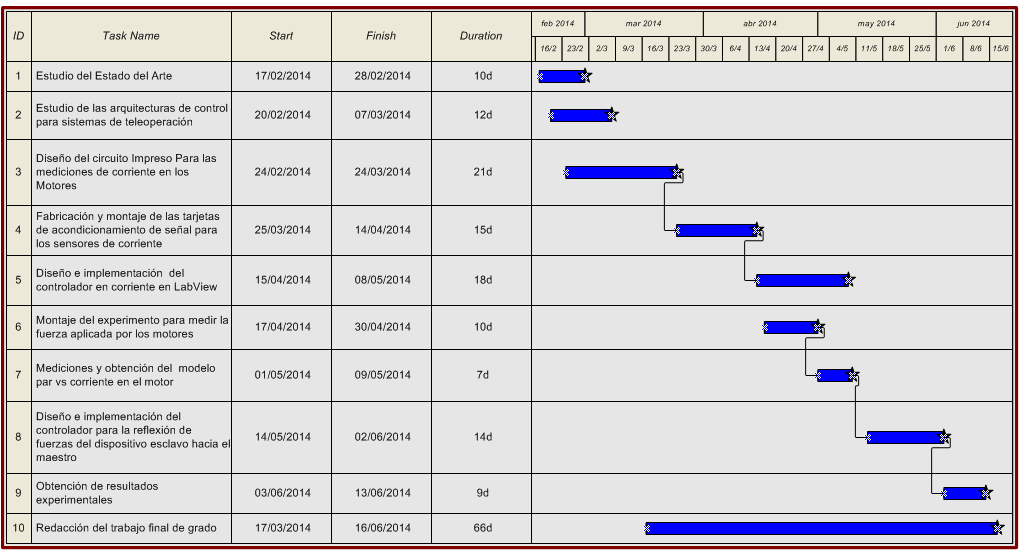
\includegraphics[scale=0.7]{FiguresP/Gant}
\end{sidewaysfigure}


%\begin{flushleft}
%\begin{frame}{Presupuesto Controlador de tiempo Real }
%
%\begin{tabular}{|c|c|c|c|c|}
% \hline
% \hline
%Conf      & Descripción    & Precio Unitario & Cantidad & Precio  \\
% \hline
% \hline
% 1  & 1      & PXI-103x and PXIe-107x Slide handle   & 0     & $\theta_1$\\
% 
% 2  & 1      & 0                                                      & 0     & 53.07 Eur\\
% 3  & 1      & 0                                                     & 0     & 53.07 Eur\\
% 4  & 1      & 0                                                     & $d_3$ & 53.07 Eur\\
% 5  & 1      & 0                                                     & 0     & 53.07 Eur\\
% 6  & 1      & 0                                                    & $d_6$ & 53.07 Eur\\
% 7  & 1      & 0                                                    & $d_6$ & 53.07 Eur\\
% 8  & 1      & 0                                            & $d_6$ & 53.07 Eur\\
% 9  & 2      & 0                                            & $d_6$ & 53.07 Eur\\
% 10 & 1      & 0                                                & $d_6$ & 53.07 Eur\\
% 11 & 4      & 0                                                & $d_6$ & 53.07 Eur\\
% 12 & 2      & 0                                                & $d_6$ & 53.07 Eur\\
% 13 & 2      & 0                                        & $d_6$ & 53.07 Eur\\
% 14 & 1      & 0                                        & $d_6$ & 53.07 Eur\\
% 15 & 1      & 0                                                & $d_6$ & 53.07 Eur\\
% \hline
% \hline
%    &        &                  &       & total          \\      
%    &        &                  &       & 16.615,64 Eur          \\      
% \hline
% \hline
%\end{tabular}
%\end{frame}
%\end{flushleft}









